%%%%%%%%%%%%%%%%%%%%%%%%%%%%%%%%%%%%%%%%%%%%%%%%%%%%%%%%%%%%%%%%%%%%%%%%
%                                                                      %
%     File: Thesis_Background.tex                                      %
%     Tex Master: Thesis.tex                                           %
%                                                                      %
%     Author: Andre C. Marta                                           %
%     Last modified :  2 Jul 2015                                      %
%                                                                      %
%%%%%%%%%%%%%%%%%%%%%%%%%%%%%%%%%%%%%%%%%%%%%%%%%%%%%%%%%%%%%%%%%%%%%%%%

\chapter{The standard model and beyond}
\label{chapter:SM}

The Standard Model (SM) is the theoretical framework that summarizes our present knowledge of particle physics. In section \ref{section:overview_SM}, we provide an overview of this model, focusing on the Higgs mechanism. In section \ref{section:BSM}, we motivate the need to explore models beyond the SM and introduce some of the most well known beyond the SM (BSM) models. In section \ref{section:Higgs_pair}, we provide a theoretical description of the production of Higgs boson pairs which is the physical process that is under study throughout this work.

%In this chapter we review the theoretical, experimental and phenomenological background that support and motivate this work. We briefly describe the Standard Model, including the Higgs mechanism, as well as introduce and motivate some Beyond the Standard Model models. We describe the process of Higgs pair production as a probe of physics both within and beyond the Standard Model (section \ref{section:theoretical}). We briefly review the Large Hadron Collider, its physics program and future upgrades and present a status of the Higgs pair production searches lead by the ATLAS and CMS experiments (section \ref{section:experimental}). We access the Higgs pair production process discovery potential both at the LHC and at future colliders based on feasibility studies (section \ref{section:pheno}). 

%%%%%%%%%%%%%%%%%%%%%%%%%%%%%%%%%%%%%%%%%%%%%%%%%%%%%%%%%%%%%%%%%%%%%%%%
\section{The Standard Model of Particle Physics}
\label{section:overview_SM}

%IDEAS FOR SECTION
%
%- Historic development +  biggest breakthroughs  \\
%- Theoretical description of SM: Symmetry group, Lagrangian, ...\\
%- Biggest successes + experimental confirmations\\
%
%- Theoretical description of Higgs mechanism: symmetry breaking + mass generation for gauge bosons\\
%- Yukawa couplings as a source of mass for leptons

The Standard Model of particle physics summarizes our present knowledge of fundamental particles and their interactions. It is formulated in the framework of Quantum Field Theory (QFT) and describes the subatomic world in terms of fields whose excitations are the particles we can detect. The particle content of the SM is summarized in figure \ref{fig:sm_particles}. Each particle is represented inside a square. The electric and color charge are shown in the right upper corner and the spin in the right lower corner. The mass of the particles are given in electron-Volt (eV) on top of each square (M standing for Million eV and G standing for Billion eV). There are two types of fundamental particles: matter particles and force carriers. 

Matter particles are the building blocks of all the matter in our world. They come in two groups, leptons and quarks. Quarks make up atomic nuclei; leptons, namely electrons and muons, can orbit atomic nuclei forming atoms. Quarks and leptons are elementary fermions which means they have half-integer spin. There are six flavors of quarks: three of the 'up type' (up, charm and top represented by $u$, $d$ and $t$) with electric charge of $+2/3$ and three of 'down type' (down, strange and bottom represented by $d$, $s$ and $b$) with electric charge of $-1/3$. Similarly, we have three leptons with charge $-1$ (electron, muon and tau represented by $e$, $\mu$ and $\tau$) and three neutral leptons (electron, muon and tau neutrinos represented by $\nu$ with the symbol of the corresponding charged lepton as subscript) that are, within the SM, massless. We can classify quarks and leptons in three generations, each composed of an up type and down type quark or of a charged lepton and the corresponding neutrino.

The force carriers, technically called gauge bosons, are particles associated with the fundamental interactions: strong, electromagnetic, weak and gravitational \footnote{The gauge boson that corresponds to the gravitational force has not yet been found. In addition we still do not have a theory that successfully describes gravitation in the framework of QFT so we will not include the gravitational force or its gauge boson in any of the following discussions. Moreover, the gravitational interaction is not relevant for the energy ranges studied.}. Each interaction can be interpreted as the result of the exchange of the corresponding gauge boson. Gluons ($g$) and the photon ($\gamma$) are the mediators of the strong and electromagnetic interactions, respectively. They are massless, electrically neutral and have spin $1$. The $W^{\pm}$ and $Z$ bosons are the mediators of the weak interaction and have a mass of $80.4$ and $91.2$ GeV, respectively. The $W^+$ and $W^-$ bosons have electric charges of $+1$ and $-1$, respectively and spin $1$. The $Z$ boson is electrically neutral and also has spin $1$. The gauge bosons can also be referred to as vector bosons because they have spin equal to one.

In addition to matter particles and gauge bosons, the theoretical formulation of the SM rests on the existence of the Higgs boson that is an electrically neutral and spin $0$ particle. It has a mass of $125$ GeV and it interacts with every particle that has mass.

%The fermions, gauge bosons and Higgs boson properties, namely, electric charge, spin and mass are summarized in Table \ref{table:SM}.

\begin{figure}[]
	\centering
	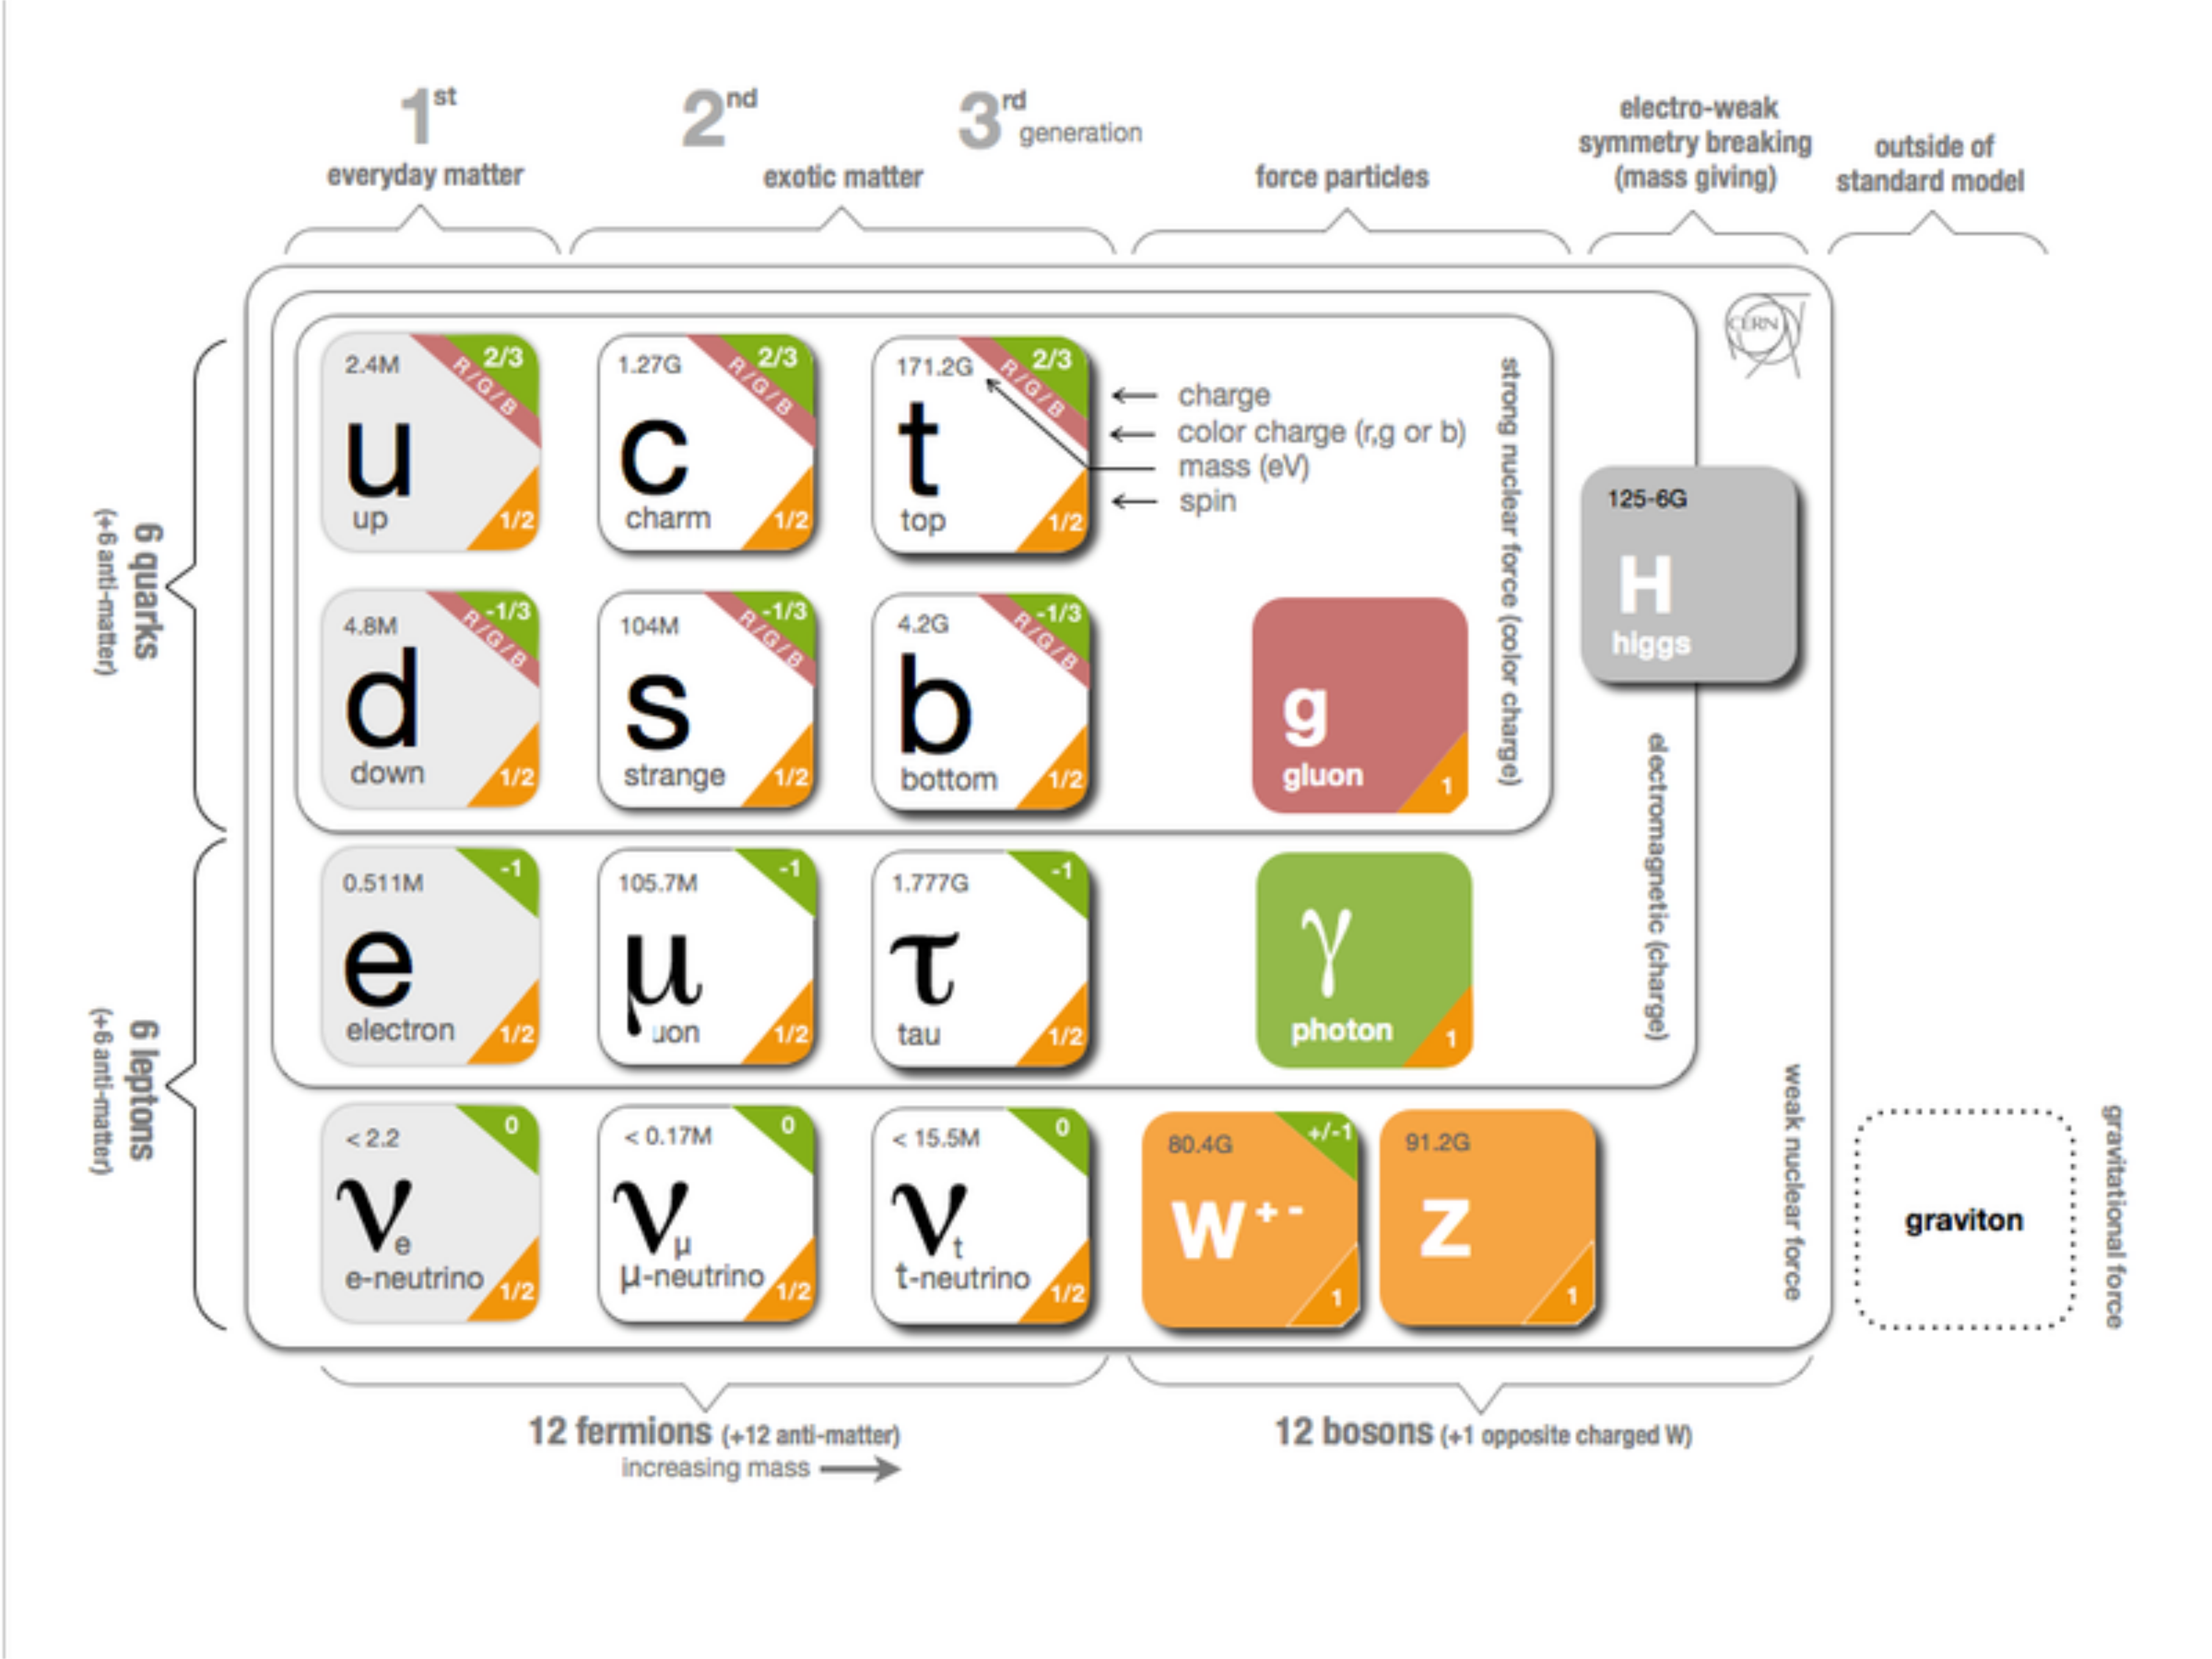
\includegraphics[trim={.5cm 1.5cm 0.5cm 0},clip,width=.8\textwidth]{./Figures/SM_CERN1.png}
	%\caption{Pictorial representation of the SM particles and their interactions. QFD stands for Quantum Flavor Dynamics and BEH stands for Brout-Englert-Higgs. Image from \cite{SMdiv}.}
	\caption{Schematic representation of the Standard Model of elementary particles. Particle are represented inside squares. The electric and color charge are shown in the right upper corner of each square. The spin is shown in the right lower corner. The mass of the particles is also shown, in electron Volt.}
	\label{fig:sm_particles}
\end{figure}

%\begin{table}
%	\centering
%	\begin{tabular}{lllll}
%		\toprule 
%		Type& Particles & Electric charge & Spin & Mass \\
%		\midrule
%		\multirow{2}{*}{Quarks} & $u$, $c$, $t$ & $2/3$ & \multirow{4}{*}{$1/2$}  & $0.0022,1.27,173.21$ GeV\\
%		  & $d$, $s$, $b$ & $-1/3$ &  & $0.0047,0.096,4.18$ GeV\\
%		\multirow{2}{*}{Leptons} & $e$, $\mu$, $\tau$ & $-1$ &  &  $0.51,105.66,1776.86$ MeV\\
%		& $\nu_e$, $\nu_{\mu}$, $\nu_{\tau}$ & $0$ &  & $<2$ eV \\
%		\midrule \midrule
%		\multirow{4}{*}{Gauge bosons} & $g$ &$0$ &\multirow{4}{*}{$1$} & $0$\\
%		 & $\gamma$ & $0$ &  &  $< 10^{-18}$ eV\\
%		 & $W^{\pm}$ & $\pm 1$& & $80.385$ GeV \\
%		& $Z$ & $0$& & $91.1876$ GeV\\
%		\midrule \midrule
%		Higgs boson & $H$ & $0$ & $0$ & $125.09$ GeV\\
%		\bottomrule
%	\end{tabular}
%	\caption{Summary of the particle content of the SM.}
%	\label{table:SM}
%\end{table}

Historically, an empirically successful quantum theory of electromagnetism, Quantum Electrodynamics (QED), was developed in the late 1940's. In the early 1950's there were high hopes that quantum theories could also be formulated for the weak and strong interactions. This is the context in which Yang-Mills theories emerged. They extend the concept of gauge theory from abelian groups, that led to the development of QED, to non-abelian gauge groups. However, the quanta of the fields predicted by these theories must be massless in order to maintain gauge invariance. Therefore, they were set aside until the 1960's when the idea of particles acquiring mass through symmetry breaking in massless theories was put forward by Goldstone \cite{Goldstone}, Nambu and Jona-Lasinio \cite{Nambu-Jona-Lasinio}. In the following paragraphs we discuss in more detail the caveats of Yang-Mills theories and the phenomenon of Spontaneous Symmetry Breaking (SSB) as the basis of the modern Higgs mechanism. We then describe this mechanism in the framework of the SM.   

On the one hand, if one takes a Yang-Mills theory, it becomes clear that it is not possible to include in the Lagrangian a mass term for the gauge bosons because it is not invariant under a gauge transformation. This would not be a problem if we just wanted to describe electromagnetic or strong interactions because the gauge bosons associated with these interactions, the photon and the gluons, are indeed massless. However, for the weak interactions this is not the case. Even before the discovery of the $Z$ and $W^{\pm}$ bosons \cite{Zdiscovery,Wdiscovery} there was experimental evidence of the short range character of the weak interactions which indicated that the corresponding gauge bosons should be massive. 

On the other hand, spontaneous symmetry breaking (SSB) is a phenomenon through which the invariance of a system under a certain symmetry group is destroyed \cite{SSB}. The system may then be invariant under a subgroup of the initial symmetry but the invariance under the original symmetry group is no longer present. In particle physics, this happens because the vacuum of the system (lowest energy states) does not share the symmetry of the Lagrangian. The SSB mechanism predicts the existence of scalar massless particles, the Nambu-Goldstone bosons, as a consequence of the Goldstone theorem \cite{Goldstone} (the number depends on the number of generators of the original and final symmetry groups). Though, when considering this mechanism we get once again massless particles which does not seem to be a step in the right direction if we wish to describe weak interactions. 

However, the real breakthrough occurs when we combine a theory with local gauge invariance with the mechanism of SSB. In this case the Nambu-Goldstone bosons do not appear and it is possible to give mass to the gauge bosons. This is the Higgs mechanism, proposed independently by P.W. Higgs \cite{Higgs}, F. Englert and R. Brout \cite{EnglertBrout} and by G. Guralnik, C. R. Hagen and T. Kibble \cite{Guralnik} in 1964. 

The SM is a non-abelian gauge theory with spontaneous symmetry breaking. It is locally invariant under the following symmetry group:

\begin{equation}
SU_{color}(3)\times SU_L(2)\times U_Y(1), 
\end{equation} 
where the $SU_{color}(3)$ group describes the strong interactions (QCD) and the $SU_L(2)\times U_Y(1)$ group describes the electroweak interactions. Here, $L$ stands for left and $Y$ stands for hypercharge. In the SM the Higgs mechanism, which we now describe, is realized in the $SU_L(2)\times U_Y(1)$ group. The Lagrangian corresponding to the Higgs and gauge sectors of this theory is given by:

\begin{equation}
\mathcal{L}=(D_{\mu}\phi)^{\dagger}(D^{\mu}\phi)-V(\phi^{\dagger} \phi)-\frac{1}{4} W_{\mu \nu}^a W^{a \mu \nu}-\frac{1}{4} B_{\mu \nu} B^{\mu \nu},
\label{eq:Lagragian}
\end{equation}
where the Higgs potential, $V(\phi^{\dagger} \phi)$, is given by:
\begin{equation}
V(\phi^{\dagger} \phi) = \mu^2 \phi^{\dagger} \phi + \lambda (\phi^{\dagger} \phi)^2.
\label{eq:higgsV}
\end{equation}
%and $W_{\mu \nu}^a~(a=1,2,3)$ and $B_{\mu \nu}$ are field strength tensors associated with the gauge fields of $SU_L(2)$ and $U_Y(1)$, $W_{\mu}^a$ and $B_{\mu}$, respectively. The covariant derivative, $D_{\mu}$, is given by
%\begin{equation}
%	D_{\mu}\equiv \partial_{\mu} + igW_{\mu}^a\frac{\tau^a}{2}+ig'B_{\mu}\frac{\mathbb{1}}{2},
%\end{equation}
%where $\tau^a$ are the Pauli matrices and $g$, $g'$ are the coupling constants of $SU_L(2)$ and $U_Y(1)$, respectively. 
$W^a_{\mu\nu}$ and $B_{\mu\nu}$ are the field tensors, defined as a function of the gauge fields of $SU_L(2)$ and $U_Y(1)$, $W^a_{\mu}~(a=1,2,3)$ and $B_{\mu}$,  respectively:

\begin{align}
	W^a_{\mu\nu}&=\partial_{\mu}W^a_{\nu}-\partial_{\nu}W^a_{\mu}-g\epsilon^{abc}W^b_{\mu}W^c_{\nu} \\
	B_{\mu\nu}&=\partial_{\mu}B_{\nu}-\partial_{\nu}B_{\mu}
\end{align}
where $g$ is the coupling constant associated with the $SU_L(2)$ group and $\epsilon^{abc}$ is the completely anti-symmetric tensor in 3 dimensions. The covariant derivative, $D_{\mu}$, is introduced to preserve local gauge invariance and is given by:

\begin{equation}
	D_{\mu}\phi = \left(\partial_{\mu} + igW^a_{\mu}T^a + i\frac{g'}{2}B_{\mu}\right)\phi.
	\label{eq:covariant_derivative}
\end{equation}
$T^a=\frac{\tau^a}{2}$ (where $\tau^a$ are the Pauli matrices) are the $SU_L(2)$ group generators in the fundamental representation and $g'$ is the coupling constant associated with the $U_Y(1)$ group.

Due to the requirement of Lorentz invariance, only the scalar field, $\phi$, can have a vacuum expectation value (VEV), $v$, different from zero \footnote{The other fields that appear in Eq. \ref{eq:Lagragian} are vector fields. If they were to acquire a VEV different from zero that would break Lorentz invariance.}. The values of $v$ are determined by the minima of the potential:
\begin{equation}
v=0 \qquad \text{or} \qquad v=\sqrt{\frac{-\mu^2}{2\lambda}}.
\end{equation}
For the equation on the right (for which we get $v\neq 0$) we only obtain a real value for $v$ (which is a requirement for the VEV of a theory) if $\mu^2<0$. Therefore we conclude that the equation on the right corresponds to $\mu^2\leq0$ while the equation on the left corresponds to $\mu^2\geq0$. In both cases $\lambda$ has to be larger than zero to guarantee that the energy is bounded from below\footnote{In a purely mathematical formulation this means that the function that represents the Higgs potential is concave upwards.} because in Eq. \ref{eq:higgsV} $\lambda$ is the coefficient of the term with the highest power in $\phi$ and therefore determines the concavity of the potential. 

The shapes of the Higgs potential for $\mu^2>0$ and $\mu^2<0$ are shown in Figures \ref{fig:higgsV}(a) and \ref{fig:higgsV}(b), respectively. For $\mu^2>0$ we have a single minimum located at $\langle\phi\rangle=0$. For $\mu^2<0$ the potential has the shape of a 'Mexican hat'. There is an infinite number of minima located in a circumference centered at zero. In this case the minima occur for $\langle\phi\rangle,\langle\phi^{\dagger}\rangle\neq 0$. Therefore the field acquires a VEV different than zero and this is what leads to the SSB.

%\begin{figure}
%	\centering
%	\begin{subfigure}{.5\textwidth}
%		\centering
%		\includegraphics[trim={0cm 1cm 0cm 2.5cm},clip,width=\linewidth]{/home/user/Desktop/5ano1sem/Tese/ProjetoMEFT/higgsV_NSB.pdf}
%		\caption{$\mu^2>0$}
%	\end{subfigure}%
%	\begin{subfigure}{.5\textwidth}
%		\centering
%		\includegraphics[trim={0cm 1cm 0cm 2.5cm},clip,width=\linewidth]{/home/user/Desktop/5ano1sem/Tese/ProjetoMEFT/higgsV_SB.pdf}
%		\caption{$\mu^2<0$}
%	\end{subfigure}
%	\caption{Shape of the Higgs potential. Spontaneous symmetry breaking happens when the potential has the shape shown on the right.}
%	\label{fig:higgsV}
%\end{figure}

\begin{figure}
	\centering
	\begin{minipage}{.5\textwidth}
		\centering
		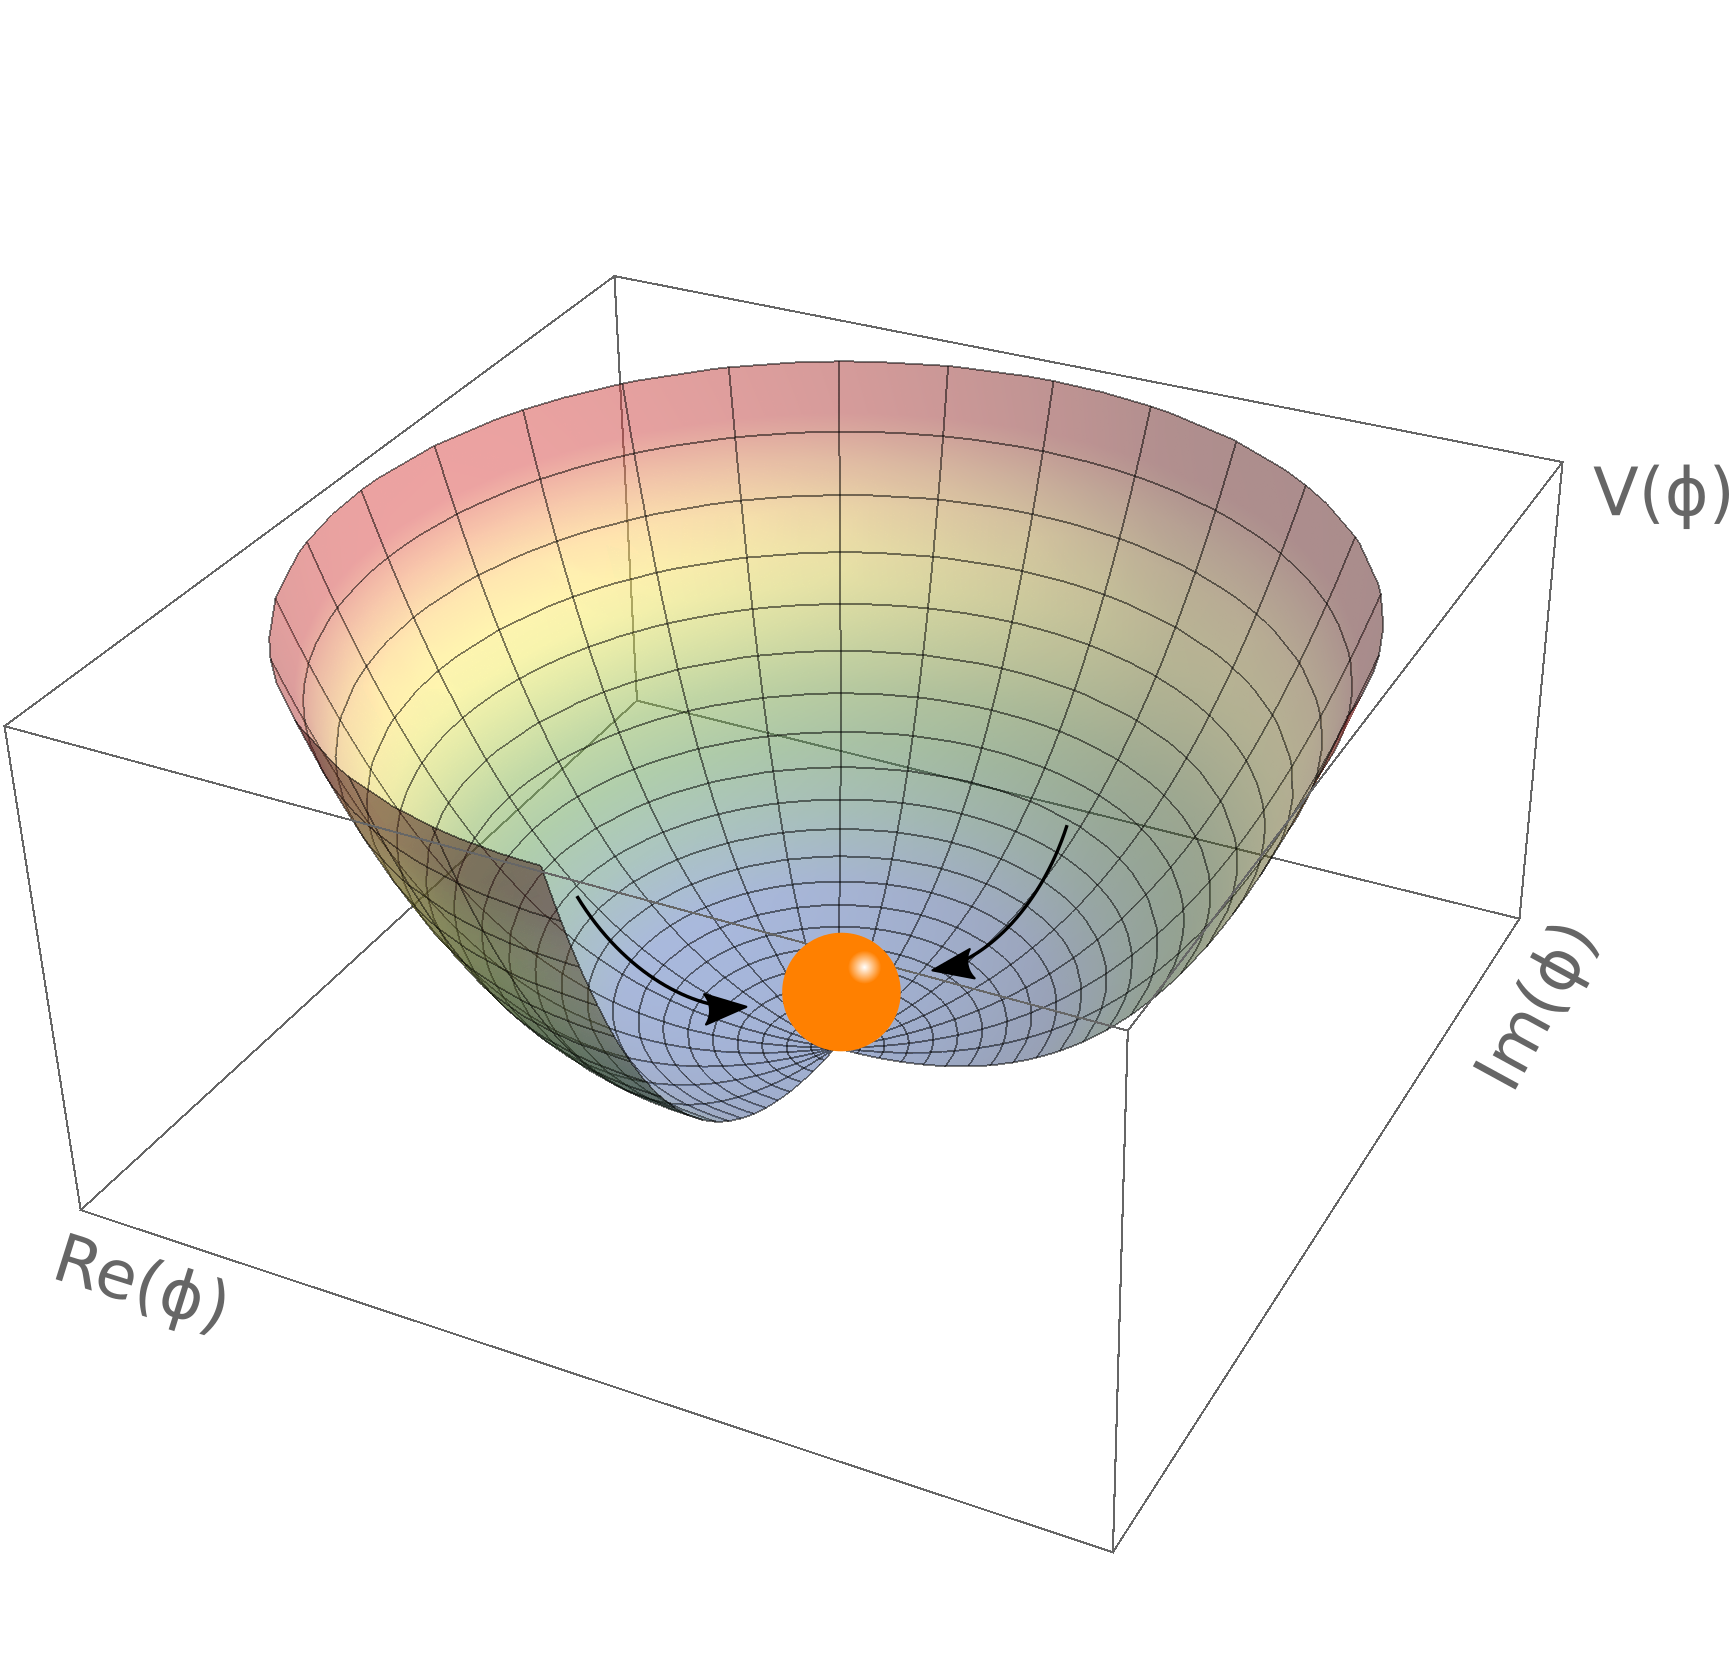
\includegraphics[trim={0cm 1cm 0cm 2cm},clip,width=\linewidth]{./Figures/HiggsV_noEWSB.png}
	\end{minipage}%
	\begin{minipage}{.5\textwidth}
		\centering
		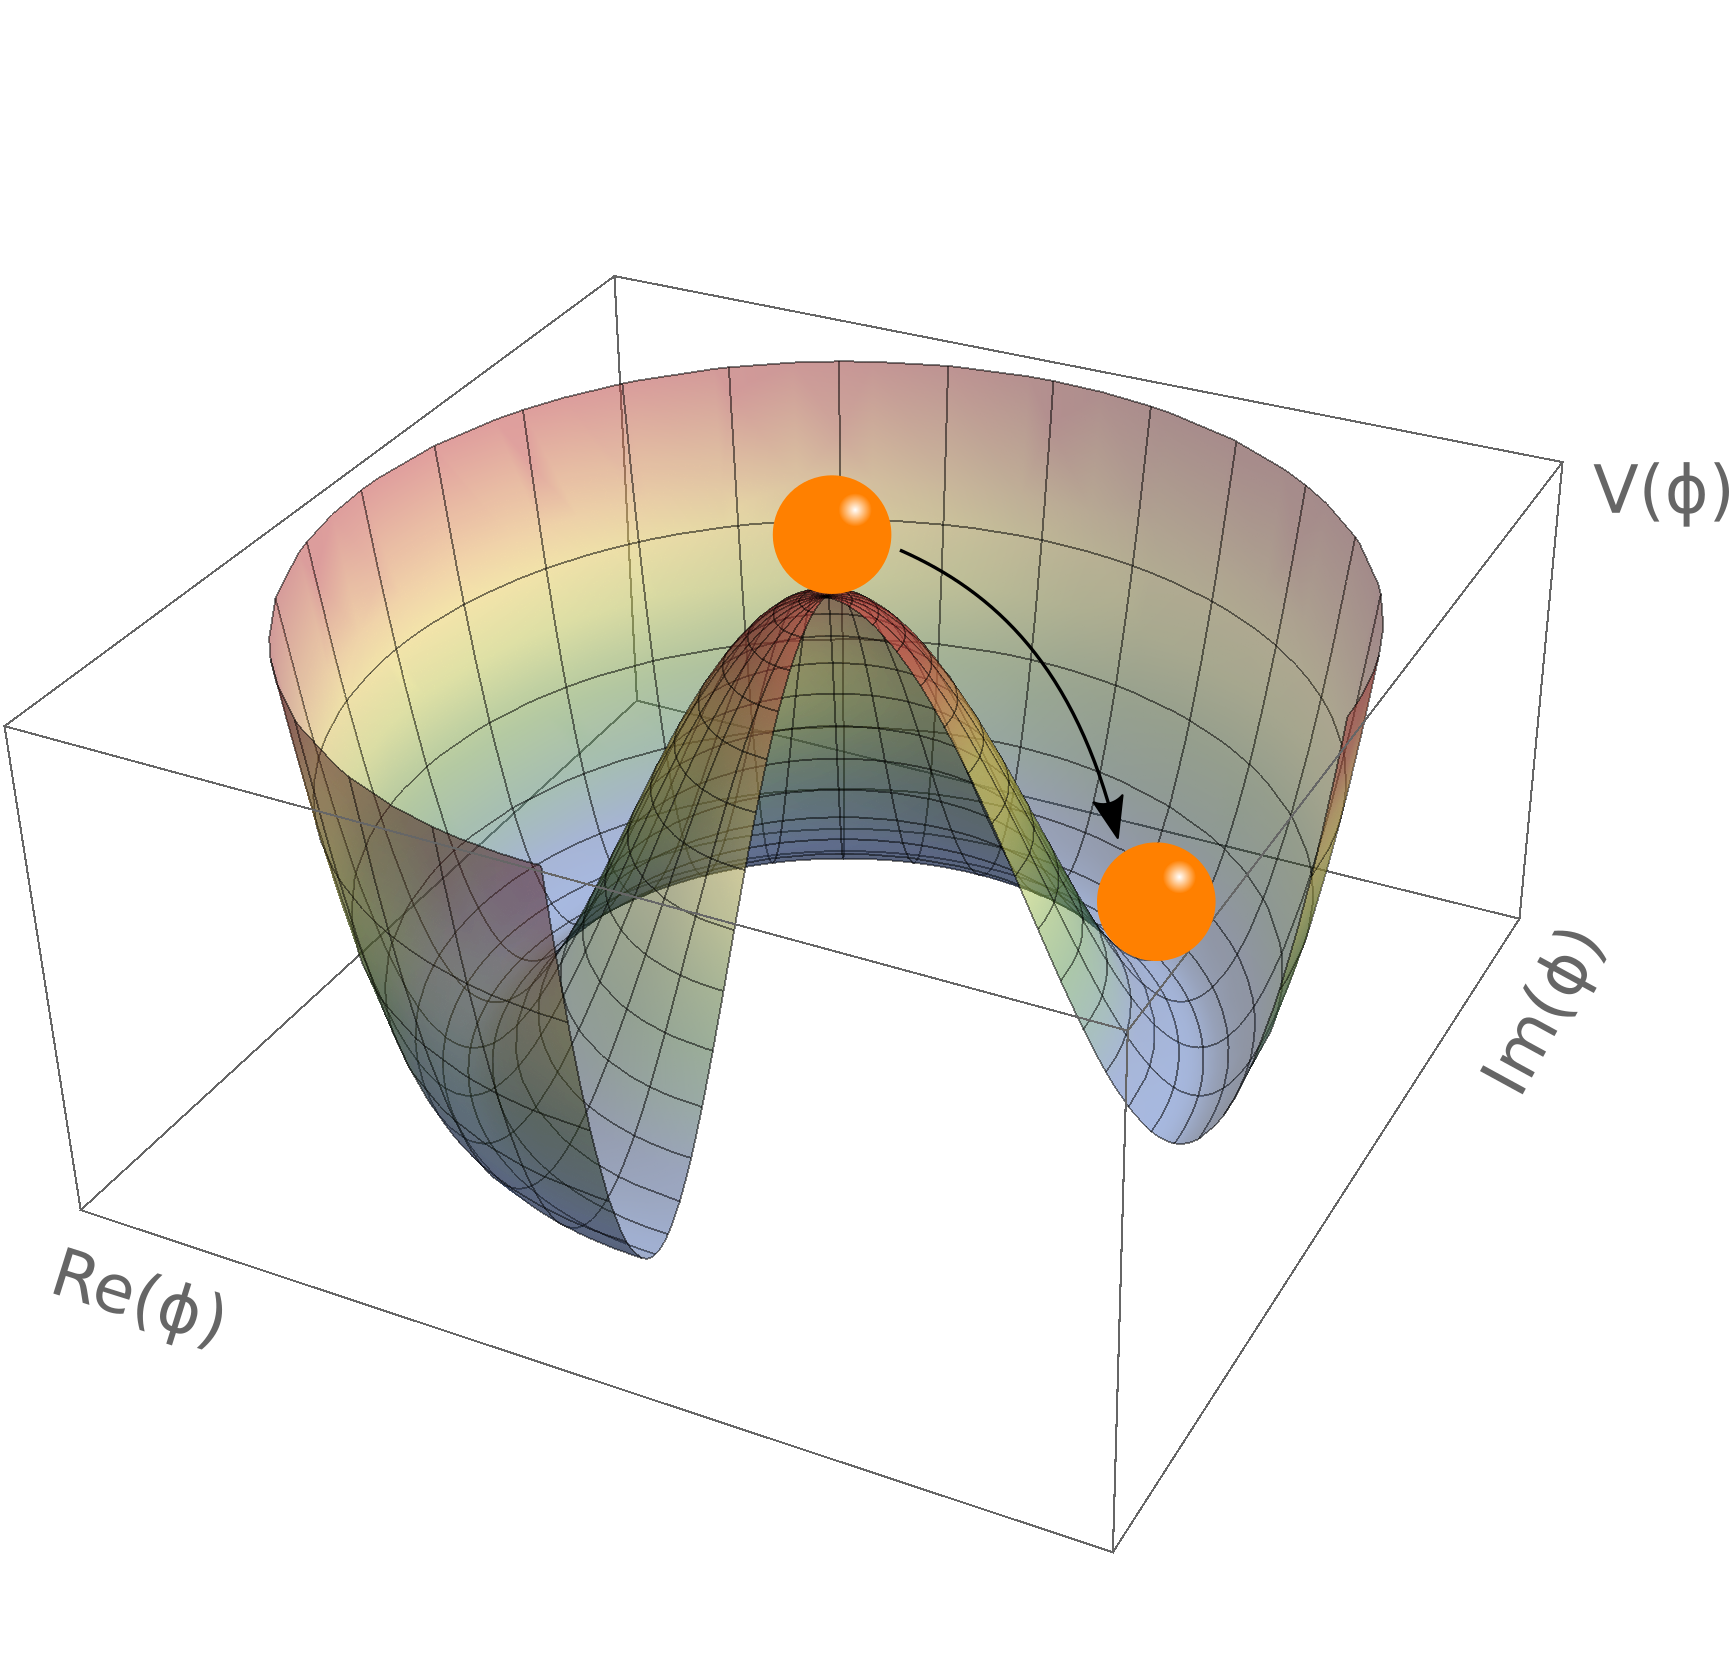
\includegraphics[trim={0cm 1cm 0cm 2cm},clip,width=\linewidth]{./Figures/HiggsV_EWSB.png}
	\end{minipage}
	
	\begin{minipage}[t]{0.5\textwidth}
		\caption*{(a)}
		%\label{fig1}
	\end{minipage}%%%
	\hfill
	\begin{minipage}[t]{0.5\textwidth}
		\caption*{(b)}
		%\label{fig2}
	\end{minipage}
	\caption{Postulated shape of the Higgs potential for $\mu^2>0$ (a) and $\mu^2<0$ (b).}
	\label{fig:higgsV}
\end{figure}

We can now write the scalar field in terms of its minimum value, $v$, and of oscillations around that minimum, $h$ (which corresponds to the Higgs field):
\begin{equation}
\phi = \begin{bmatrix}
0 \\
v+\frac{h}{\sqrt{2}} \\
\end{bmatrix} \qquad (\textit{unitary gauge}).
\label{eq:higgs_field}
\end{equation}
If we expand the first term of the Lagrangian shown in Eq. \ref{eq:Lagragian} using Eq. \ref{eq:covariant_derivative} and Eq. \ref{eq:higgs_field} and taking into consideration that $W^a_{\mu}T^a$ represents a sum over all values of $a$ we get

\begin{align}
	\mathcal{L} = \frac{1}{4}\left(v^2+\frac{h^2}{2}+\frac{2}{\sqrt{2}}vh\right) \left[g^2\left(W^1_{\mu}W^{1\mu}+W^2_{\mu}W^{2\mu}+W^3_{\mu}W^{3\mu}\right)-2gg'B^{\mu}W^3_{\mu}+g'^2 B_{\mu}B^{\mu}\right] + ...~.
	\label{eq:Lagrangian_transform}
\end{align}
We see that for the $W^1_{\mu}$ and $W^2_{\mu}$ fields we have only terms that are quadratic in these fields. These correspond to mass terms. However, for the $W^3_{\mu}$ and $B_{\mu}$ fields there is a term that mixes the two fields. To obtain the physical states of the theory we need to transform these fields in order to get rid of the mixing term which is not physical. We can start by writing the last three terms of Eq. \ref{eq:Lagrangian_transform} in a matrix form and diagonalize the corresponding matrix:
\begin{equation}
\begin{bmatrix}
g^2 & -gg' \\
-gg' & g'^2 \\
\end{bmatrix}
\begin{bmatrix}
W^3_{\mu} \\
B_{\mu} \\
\end{bmatrix}
\xrightarrow{\text{Diagonalization}}
\begin{bmatrix}
0 & 0 \\
0 & g^2+g'^2 \\
\end{bmatrix}
\begin{bmatrix}
A_{\mu} \\
Z_{\mu} \\
\end{bmatrix}.
\label{eq:gauge_matrix}
\end{equation}
$A_{\mu}$ and $Z_{\mu}$ are the physical fields that are related with $W^3_{\mu}$ and $B_{\mu}$ by means of a rotation matrix:
\begin{equation}
\begin{bmatrix}
A_{\mu} \\
Z_{\mu} \\
\end{bmatrix}=
\begin{bmatrix}
\cos\theta_W & -\sin\theta_W \\
\sin\theta_W & \cos\theta_W \\
\end{bmatrix}
\begin{bmatrix}
W^3_{\mu} \\
B_{\mu} \\
\end{bmatrix}
\end{equation}
where $\theta_W$ is the Weinberg angle.
By inverting this relation we can write $W^3_{\mu}$ and $B_{\mu}$ as a function of $A_{\mu}$ and $Z_{\mu}$. Replacing in Eq. \ref{eq:Lagrangian_transform} and imposing that the $A_{\mu}$ field has zero mass we can determine $\theta_W$: $\tan\theta_W=\frac{g'}{g}$. The Lagrangian of Eq. \ref{eq:Lagrangian_transform} takes then the form
\begin{equation}
	\mathcal{L}=\frac{1}{2}\left(v^2g^2\right)\left(W^1_{\mu}W^{1\mu}+W^2_{\mu}W^{2\mu}\right)+\frac{1}{2}\left(v^2\left[g^2+g'^2\right]\right)Z_{\mu}Z^{\mu}+...~,
\end{equation}
where we show only the mass terms for the gauge bosons. Note that, by construction, there is no mass term for $A_{\mu}$ which allows us to identify this field with the photon. $W^1_{\mu}$ and $W^2_{\mu}$ are related to the $W^{\pm}$ boson and $Z_{\mu}$ corresponds to the $Z$ boson. We have shown that it is the fact that $v\neq0$ that allows for the existence of non-zero mass terms for the $W^{\pm}$ and $Z$ bosons.

If we now expand the second term of the Higgs potential (Eq. \ref{eq:higgsV}) using Eq. \ref{eq:higgs_field} we get, among other terms,
\begin{equation}
\mathcal{L}=-h^3\sqrt{-\mu^2 \lambda} - h^4\lambda+...~.
\label{eq:higgs_couplings}
\end{equation}
These terms encode the Higgs self interactions and represent, respectively, the three and four point interactions. We see that the coupling constants of these interactions depend on the parameters of the Higgs potential, $\mu^2$ and $\lambda$.

In addition to being responsible for giving mass to the gauge bosons, the Higgs field is also responsible for the mass of the fermions. However, the mechanism through which this occurs is fundamentally different. In the case of fermions, the mass terms are placed explicitly in the Lagrangian:

\begin{equation}
	\mathcal{L}_{\text{fermions}}=G_1 \overline{L}\phi R + G_2 \overline{L}\phi_c R + \text{hermitian conjugate}
	\label{eq:fermions_mass}
\end{equation}
where $L$ denotes a left-handed fermion doublet and $R$ denotes a right-handed fermion singlet. Here, left and right refer to helicity states. $G_1$ and $G_2$ are arbitrary coupling constants that can be written in terms of the fermion's mass and the VEV. $\phi$ is given by Eq. \ref{eq:higgs_field} and $\phi_c$ is given by (after the spontaneous symmetry breaking and in the unitary gauge):

\begin{equation}
	\phi_c=\begin{bmatrix}
	v+\frac{h}{\sqrt{2}} \\
	0 \\
	\end{bmatrix}.
\end{equation}

We now take a quick detour to motivate why fermions are represented as chiral states (left and right) of the $SU_L(2)$ symmetry. We base this discussion on Ref. \cite{rute}. In the context of the unification of the electromagnetic and weak forces, formalized by Weinberg, Glashow and Salam in 1961, both interactions are interpreted as manifestations of the electroweak force. Weak charged currents are axial vector currents which means they couple only to left handed fermions while weak neutral currents, as well as QED, couple to both helicity states. This suggested that fermions were better represented as left-handed doublets and right-handed singlets of the $SU_L(2)$ symmetry group. The left handed doublets, $L$, are defined as:
\begin{equation}
L:\begin{pmatrix}
\nu_l \\
l \\
\end{pmatrix}_L,
\begin{pmatrix}
u \\
d' \\
\end{pmatrix}_L
\end{equation}
where $l$ represents an electron, muon or tau, $u$ is any quark of the up type and $d'$ is a quark of the down type. The right-handed states, $R$, are singlets, define as:
\begin{equation}
	R: l_R,u_R,d'_R.
\end{equation} 
In 1956, C. S. Wu \textit{et al.} showed that the weak interaction violates parity conservation \cite{wu}. In 1958, M. Goldhaber \textit{et al.} conducted an experiment that showed that neutrinos are left-handed and anti-neutrinos are right-handed \cite{goldhaber} which is why the SM does not include a right-handed state for neutrinos. 
We can now continue the discussion of the mass generation mechanism for fermions.

The first term in Eq. \ref{eq:fermions_mass} gives mass to down type fermions (electron, muon, tau, down, strange and bottom quarks) and the second to up type fermions (up, charm and top quarks). In addition, these terms give rise to the interaction terms between the Higgs field and the fermions. Take, as an example, $\overline{L}=(\overline{t}, \overline{b})_L$ and $R=b_R$. For the first term of Eq. \ref{eq:fermions_mass} we get:

\begin{equation}
	G_1 \overline{L}\phi R = G_1 ~(\overline{t}, \overline{b})_L \begin{bmatrix}
	0 \\
	v+\frac{h}{\sqrt{2}} \\
	\end{bmatrix} b_R = G_1 v ~\overline{b}_L b_R + \frac{G_1}{\sqrt{2}} \overline{b}_L b_R h.
\end{equation}
The first term is the mass term for b quarks. Therefore we can redefine $G_1 v = m_b$ and obtain:
\begin{equation}
	G_1 \overline{L}\phi R=m_b \overline{b}_L b_R + \frac{m_b}{v\sqrt{2}} \overline{b}_L b_R h.
\end{equation}
The second term gives the interaction between the Higgs boson and the fermions, in this case, the b quarks. The strength of this interaction is directly proportional to the mass of the corresponding fermion.

In the SM formalism, neutrinos as massless particles. However, there is no reason why they cannot acquire mass through a mechanism similar to the one we just described. Nonetheless, the usual argument is that it would be unnatural for the same mechanism to produce the mass of very heavy particles, such as the top quark, and the mass of very light particle, such as the neutrinos. Therefore, BSM models that try to explain the mass generation for neutrinos usually resort to a different mechanism.

%\begin{equation}
%	\mathcal{L}_{leptons}=\sum_f \overline{\Psi}_f \left(i\slashed{D}-M\right)\Psi_f,
%\end{equation}
%where $f$ represents any fermion, $\Psi_f$ is a Dirac spinor $\slashed{D}$ is given by ...  and $M$ is a mass matrix. 

The SM has delivered extremely accurate predictions about the existence and properties of new particles which make it a very successful theory. It predicted the existence of the W and Z bosons \cite{Glashow-Weinberg-Salam}, the gluon, the charm and top quarks and the Higgs boson \cite{Higgs,EnglertBrout,Guralnik}. In addition, the SM prediction for the value of the anomalous magnetic dipole moment of the electron (calculated up to order $\alpha^5$) agrees with the measured value up to the $11^{th}$ decimal place, making it the most precise measurement in science.

%
%A reference can be cited in any of the following ways:
%%
%\begin{itemize}
%  \item Citation mode \#1 - \quad \cite{jameson:adjointns}
%  \item Citation mode \#2 - \quad \citet{jameson:adjointns}
%  \item Citation mode \#3 - \quad \citep{jameson:adjointns}
%  \item Citation mode \#4 - \quad \citet*{jameson:adjointns}
%  \item Citation mode \#5 - \quad \citep*{jameson:adjointns}
%  \item Citation mode \#6 - \quad \citealt{jameson:adjointns}
%  \item Citation mode \#7 - \quad \citealp{jameson:adjointns}
%  \item Citation mode \#8 - \quad \citeauthor{jameson:adjointns}
%  \item Citation mode \#9 - \quad \citeyear{jameson:adjointns}
%  \item Citation mode \#10 - \quad \citeyearpar{jameson:adjointns}
%\end{itemize}
%%
%Several citations can be made simultaneously as \citep{nocedal:opt,marta:ijcfd}. \\
%
%This is often the default bibliography style adopted (numbers following the citation order), according to the options:\\
%{\tt \textbackslash usepackage\{natbib\}} in file {\tt Thesis\_Preamble.tex},\\
%{\tt \textbackslash bibliographystyle\{abbrvnat\}} in file {\tt Thesis.tex}.\\
%
%Notice however that this style can be changed from numerical citation order to authors' last name with the options: \\
%{\tt \textbackslash usepackage[numbers]\{natbib\}} in file {\tt Thesis\_Preamble.tex},\\
%{\tt \textbackslash bibliographystyle\{abbrvunsrtnat\}} in file {\tt Thesis.tex}. \\
%
%Multiple citations are compressed when using the {\tt sort\&compress} option when loading the {\tt natbib} package as {\tt \textbackslash usepackage[numbers,sort\&compress]\{natbib\}} in file {\tt Thesis\_Preamble.tex}, resulting in citations like \citep{marta:ijcfd1,marta:ijcfd2,marta:ijcfd3,marta:ijcfd4}.

\subsection{Higgs pair production}
\label{section:Higgs_pair}

%IDEAS FOR SECTION
%
%- Main production process and Feynman diagrams \\
%- Computation of cross section + dependency with COM energy and triple coupling\\
%- Sensitivity to shape of Higgs potential\\
%- Conclude and motivate why this process should be studied (within and beyond SM)

Within the SM there are still some processes that have not been measured. One of these is the production of pairs of Higgs bosons. The experimental challenges and efforts related to this process are discussed in section \ref{section:previous_searches}. Here we provide a theoretical description of the process.

At the Large Hadron Collider (LHC), the main production process of Higgs pairs is gluon-gluon fusion (ggF). Higgs pairs can also be produced through vector boson ($V$) fusion (VBF), in association with a pair of top quarks ($t\overline{t}h$) or through Higgs strahlung ($Vh$) \footnote{In this process, at LO, a Higgs boson is radiated from a vector boson}. At a center of mass (CM) energy of $\sqrt{s}=13$ TeV, the ggF production process has a cross section approximately seventeen times larger than the next most commom production process which is VBF (approximately $30$ fb \textit{versus} $1.6$ fb \cite{hhxsNLO}). Therefore it is the dominant contribution when we study inclusive production. For this reason we focus the following discussion on this production mode. The leading order Feynman diagrams for Higgs pair production via ggF are shown in figure \ref{fig:higgs_pair}. 

%\footnote{There are no tree level diagrams diagrams that contribute to this process. Therefore, the leading order diagrams are at on loop order.}

%\begin{table}
%	\centering
%	\begin{tabular}{lll}
%		\toprule 
%		& \multicolumn{2}{c}{Cross section [pb]} \\
%		Production mode & $14$ TeV & $100$ TeV  \\
%		\midrule
%		ggF & $50.3$ & $740.0$\\
%		\rowcolor{black!7} VBF & $4.4$ & $82.0$\\
%		$t\overline{t}h$ & $0.6$ & $37.9$ \\
%		\rowcolor{black!7} $Zh$ & $0.9$ & $11.3$\\
%		$Wh$ & $1.6$ & $15.9$ \\
%		\bottomrule
%	\end{tabular}
%	\caption{Cross sections in pb for the different Higgs production processes at $14$ and $100$ TeV.}
%	\label{table:Hprod}
%\end{table}

%The diagrams interfere destructively which is indicated by the minus sign between them.

The diagram on the right has an off-shell (virtual) Higgs boson, $h^*$, that couples to gluons by the usual heavy quark triangle (same mechanism as in single Higgs production). $h^*$  then decays to two on-shell Higgs bosons. This diagram contains the three point interaction between Higgs bosons and therefore it is the one that allows us to probe this coupling. In the diagram on the left, the two Higgs bosons couple to the gluons by a box of heavy quarks and are directly radiated from a quark. The largest contributions for these quantum loops come from heavy quarks, such as the top and bottom, because the coupling constant of the Higgs boson to fermions is directly proportional to the fermions mass (see section \ref{section:overview_SM}).

\begin{figure}[h]
	\centering
	\feynmandiagram[baseline=(current bounding box.center),large, layered layout,horizontal=a to b] {
		% Draw the top and bottom lines
		i1 -- [gluon, edge label'=\(g\)] a-- [anti fermion] b-- [scalar, edge label'=\(h\)] f1,
		i2 -- [gluon, edge label'=\(g\)] c-- [fermion] d-- [scalar, edge label'=\(h\)] f2,
		% Draw the two internal fermion lines
		{ [  same layer	] a -- [fermion] c },
		{ [  same layer] b -- [anti fermion] d},
	};\qquad \--- \qquad
	\feynmandiagram [baseline=(current bounding box.center),large, horizontal=e to f] {
		a -- [gluon, edge label'=\(g\)] b -- [anti fermion] c -- [gluon, edge label'=\(g\)] d,
		b -- [fermion] e -- [fermion] c,
		e -- [scalar, edge label'=\(h^*\)]  f,
		h -- [scalar, edge label'=\(h\)] f -- [scalar, edge label'=\(h\)] i,
		a -- [opacity=0] d,
	}; 
	\caption{Feynman diagrams of Higgs pair production from gluon fusion. Triple vertex diagram (left) and box diagram (right). The minus sign between the diagrams indicates that they interfere destructively.}
	\label{fig:higgs_pair}
\end{figure}


The amplitudes for the box, $\mathcal{M}_{\Box}$, and triangle, $\mathcal{M}_{\triangle}$, diagrams scale as \cite{FCCyellow}:
\begin{equation}
\mathcal{M}_{\Box} \sim \frac{\alpha_s}{4\pi} y_t^2, \qquad \mathcal{M}_{\triangle} \sim \lambda_{hhh} \frac{\alpha_s}{4\pi} y_t^2 \frac{m_h^2}{\hat{s}}\Big(\log \frac{m_t^2}{\hat{s}} + i\pi\Big)^2
\label{eq:hh_M}
\end{equation}
where $\hat{s}$ is the CM energy, $y_t$ is the Yukawa coupling of the top quark, $\alpha_s$ is the eletroweak coupling constant, $\lambda_{hhh}$ is the coupling constant of the Higgs boson three point self-interaction and $m_h, m_t$ are the masses of the Higgs boson and top quark.

At a CM energy of $\sqrt{s}=13$ TeV the cross section for Higgs pair production, as predicted by NLO calculations, is very small, approximatelly $30~\text{fb}$ \cite{hhxsNLO}. It is suppressed due to the destructive interference between the LO diagrams that leads to a $\sim 50\%$ supression of the total cross section \cite{FCCyellow}. Furthermore, the cross section of the triangle diagram is smaller that the one of the box diagram, approximately $4$~fb compared to $30$~fb \footnote{These values are obtained using MadGraph5. They are shown here to give a rough estimate of the difference between the values of the cross sections  of both diagrams.}, and it is strongly suppressed for larger values of the CM energy which can be seen directly from the expression of the amplitude in Eq. \ref{eq:hh_M}. This means that the Higgs trilinear coupling mostly affects the Higgs pair production at threshold. A variable that is sensitive to these effects is the invariant mass of the Higgs pair. The tail of this distribution (high invariant mass of the Higgs pair), however, is mostly determined by the box diagram contribution \cite{FCCyellow}.  

The LO calculation for the cross section of Higgs pair production has been performed, for example, in Ref. \cite{HHxs_LO}. A value of the order of $10$~fb is reported. The NLO calculation is a theoretical challenge: several two-loop diagrams that take into account virtual and real radiation have to be considered. In addition, top quark mass effects can be included in various approximations. This leads to corrections with different signs which suggests that the uncertainty on the cross section due to top quark mass effects are of the order of $\pm 10\%$ at NLO. Therefore, a calculation including the full top mass dependence was of the utmost importance. This result became available recently \cite{HHcalc_top}:
\begin{equation}
\sigma^{\text{NLO}}_{gg\rightarrow hh} = 27.80^{+13.8\%}_{-12.8\%}(\text{scale})\pm 0.3\%(\text{stat.})\pm 0.1\% (\text{int.})~\text{fb}
\end{equation}
where the dependence of the result on the variation of the scales by a factor of two around the central scale, the statistical error coming from the limited number of phase space points evaluated and the error coming from the numerical integration of the amplitude are shown. 

This result shows that the introduction of NLO contributions produces a significantly different result. Therefore the inclusion of such effects is necessary if we wish to obtain an accurate result that can be compared to experimental values. The analytical expressions for the NLO cross section are long and complex so we abstain from reproducing them here. Nonetheless, the LO cross section can be written in a compact form and it allows us to discuss some key features of the process. Therefore, we will present it here, based on Refs. \cite{HHxs_LO,HHxs_LO1}.

The partonic LO cross section for $gg\rightarrow hh$ can be written
\begin{equation}
\hat{\sigma}^{\text{LO}}_{gg\rightarrow h} (\hat{s}) \sim \int_{\hat{t}_-}^{\hat{t}_+}~d\hat{t}~\left(|C_{\bigtriangleup}F_{\bigtriangleup}+C_{\Box}F_{\Box}|^2+|C_{\Box}G_{\Box}|^2\right)
\end{equation}
where $\hat{s}$ and $\hat{t}$ are the Mandelstam variables and, in addition, $\hat{s}$ can be identified with the square of the partonic CM energy of the process. The integration limits, $\hat{t}_{\pm}$, are derived from a momentum parametrization in the CM frame, leading to $\hat{t}_{\pm}=m_h^2-\frac{\hat{s}}{2}(1\mp \beta_h)$, where $\beta_h^2=1-4\frac{m_h^2}{\hat{s}}$ and $m_h$ is the mass of the Higgs boson \cite{HHxs_LO1}. $F_{\bigtriangleup}$, $F_{\Box}$ and $G_{\Box}$ are form factors whose full expressions can be found, for example, in Ref. \cite{HHxs_LO}. $C_{\bigtriangleup}$ and $C_{\Box}$ can be interpreted as generalized couplings and are given by
\begin{equation}
C_{\bigtriangleup}=\lambda_{hhh}\frac{m_Z^2}{\hat{s}-m_h^2}, \qquad C_{\Box}=1,
\end{equation}
where $m_Z$ is the mass of the $Z$ boson.
If we take the limit $m_Q^2 \gg \hat{s}\sim m_h^2$ (where $m_Q$ is the mass of the quarks that contribute to the quantum loops) we can get simple expressions for the remaining form factors:
\begin{equation}
F_{\bigtriangleup}=\frac{2}{3} + \mathcal{O}(\hat{s}/m_Q^2), \qquad F_{\Box}=-\frac{2}{3} + \mathcal{O}(\hat{s}/m_Q^2), \qquad G_{\Box}=\mathcal{O}(\hat{s}/m_Q^2).
\end{equation}
In this limit, the partonic cross section is simply given by 
\begin{equation}
\hat{\sigma}^{\text{LO}}_{gg\rightarrow hh}(\hat{s}) \sim \int_{\hat{t}_-}^{\hat{t}_+}~d\hat{t}~ |\lambda_{hhh}\frac{m_Z^2}{\hat{s}-m_h^2}-1|^2.
\label{eq:xsparton}
\end{equation}

%To get the total cross section we need to integrate over the Parton Distributions Functions (PDFs). Defining the luminosity function as
%\begin{equation}
%\frac{d\mathcal{L}_{ij}}{d\tau} = \sum_{ij}\int_{\tau}^{1}\frac{dx}{x}f_i(x,\mu_F)f_j\left(\frac{\tau}{x},\mu_F\right)
%\end{equation}
%
%the total cross section reads
%\begin{equation}
%\sigma_{gg\rightarrow hh}^{\text{LO}}=\int_{\tau_0}^{1}~d\tau~\frac{d\mathcal{L}_{gg}}{d\tau} ~\hat{\sigma}^{\text{LO}}_{gg\rightarrow hh}(\hat{s}=\tau s),
%\label{eq:fullxs}
%\end{equation}
%where $s$ is the square of the hadronic CM energy, $\tau_0=4m_h^2/s$ and $\mu_F$ is the factorization scale.

There are two important points that are worth discussing. Firstly, the total cross section has terms that are proportional to the Higgs triple couling, $\lambda_{hhh}$, which can be read directly from Eq. \ref{eq:xsparton}. On the one hand, this means that measuring this process gives us access to the value of $\lambda_{hhh}$ and therefore provides valuable insight into the shape of the Higgs potential and ultimately into the EWSB mechanism in the SM. On the other hand, if $\lambda_{hhh}$ has a value that is different from the one predicted by the SM, that will affect the measured value of the cross section and can lead to hints of new physics. 

Secondly, although this is not evident from Eq. \ref{eq:xsparton}, the cross section for di-Higgs production increases with $\hat{s}$. This can be seen in figure \ref{fig:HHxs_s} that shows the variation of the total (integrated) NLO cross section with the CM energy for the six largest production channels. Note that increasing the CM energy from $13$ to $100$ TeV increases the inclusive cross section by approximately two orders of magnitude which is a consequence of the increased phase space that becomes available.

\begin{figure}[]
	\centering
	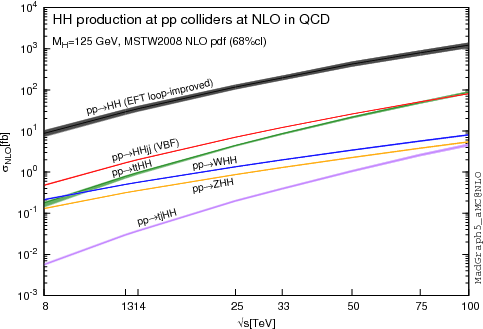
\includegraphics[width=0.6\textwidth]{./Figures/HH-xsec.png}
	\caption{Total cross sections at NLO in QCD for the six largest HH production channels at pp colliders. The thickness of the lines corresponds to the scale and PDF uncertainties added linearly.}
	\label{fig:HHxs_s}
\end{figure}

Therefore, the increase in the cross section of rare processes, such as Higgs pairs production, as the CM energy of collision experiments increases supports the claim that future colliders, with higher CM energies, might be our chance of discovering and precisely studying these processes.

%Nonetheless, if we take the limit $m_Q^2 \gg \hat{s}\sim M_H^2$ we can get simple expressions for the form factors:
%\begin{equation}
%	F_{\bigtriangleup}=\frac{2}{3} + \mathcal{O}(\hat{s}/m_Q^2), \qquad F_{\Box}=-\frac{2}{3} + \mathcal{O}(\hat{s}/m_Q^2), \qquad G_{\Box}=\mathcal{O}(\hat{s}/m_Q^2).
%\end{equation}
%In this limit, the differential cross section is given by 
%\begin{equation}
%	\frac{d\hat{\sigma}}{d\hat{t}} \sim |\lambda_{hhh}\frac{M_Z^2}{\hat{s}-M_H^2}-1|^2.
%\end{equation}
%\begin{figure}[h]
%	\centering
%	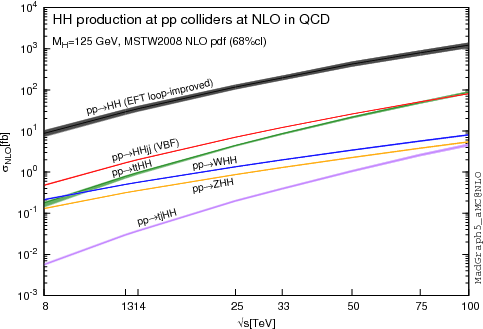
\includegraphics[width=0.7\textwidth]{./Figures/HH-xsec.png}
%	\caption{Total cross sections at the NLO in QCD for the six largest HH production channels at pp colliders. The thickness of the lines corresponds to the scale and PDF uncertainties added linearly.}
%	\label{fig:hh_xsec}
%\end{figure}

%%%%%%%%%%%%%%%%%%%%%%%%%%%%%%%%%%%%%%%%%%%%%%%%%%%%%%%%%%%%%%%%%%%%%%%%
\section{Going beyond}
\label{section:BSM}
%
%IDEAS FOR SECTION
%
%- Why we need to study physics BSM (motivation: theoretical+experimental)\\
%- Brief description of most well known and well studied BSM models that include changes in the Higgs sector, predict heavier Higgs \\
%- How these can be probed using Higgs pair production

Despite the success of the SM, there is evidence that indicates that it cannot be the final theory of particle physics. This led to the development of alternative models that extend the SM but that can still reproduce its successful predictions. These are referred to as Beyond the Standard Model (BSM) models. 

On the one hand, there are several pieces of experimental evidence that the SM cannot explain. These include the nature of dark matter, postulated to explain the experimental observations of the velocity of far away galaxies \cite{DM}, the asymmetry between matter and anti-matter in the present Universe \footnote{Or why do we live a local in an Universe made mostly out of matter?} and the fact that neutrinos oscillate between flavors which implies that they have a non-zero mass. This phenomenon was measured independently by two collaborations, the Super-Kamiokande and the Sudbury Neutrino Observatory (SNO), in 1998 and 2001-2002, respectively, \cite{neutrinosSuperK,neutrinosSNO1,neutrinosSNO2}.

On the other hand, its theoretical formulation also has some weaknesses: it accurately describes particles interactions at the electroweak scale ($\sim 246$~GeV) but it does not include gravity which means it cannot be valid at the Planck scale ($\sim 10^{19}$~GeV) where gravity cannot be overlooked; it has a lot (over $20$) of free parameters whose values have to be tuned to fit experimental observations, and there is a large discrepancy between the mass scales associated with the electroweak and gravitational interactions (this is one of the simplest formulations of what is known as the hierarchy problem).

When faced with these weaknesses, or rather hints of incompleteness, the theoretical community put a great effort into the development of models that add new ingredients to the SM. In the following paragraphs we introduce and briefly describe some of the most well studied (both theoretically and experimentally) BSM models. We follow the discussion presented in Ref. \cite{BSM_motivation} as a starting point.

It is a well known consequence of renormalization in QFT that the coupling constants become dependent on the energy scale at which the theory is probed. As the energy scale increases the $U_Y(1)$ coupling constant gets larger while the $SU_L(2)$ and $SU_{color}(3)$ coupling constants get smaller. If one extrapolates far enough these become nearly equal at an energy scale of approximately $10^{15}$~GeV. Although this matching is far from perfect, it sparked the idea that these three forces could be unified at an energy scale of $10^{15}$~GeV. Grand Unification Theories (GUT) try to combine $SU_{color}(3)\times SU_L(2)\times U_Y(1)$ into a larger symmetry group.

Supersymmetric (SUSY) models introduce a new symmetry that links fermions and bosons. For each boson(fermion) of the SM it introduces a fermionic(bosonic) partner. Apart from spin, the supersymmetric partners would share the same mass and quantum numbers. Since we have not found any supersymmetric particles in the LHC this means that supersymmetry is necessarily a broken symmetry and, if they exist, new particles should have a larger mass (outside of the present reach of the LHC) than their SM partners. SUSY models were introduced because they offer a natural fix for the hierarchy problem. In addition, the Minimal Supersymmetric extension of the SM (MSSM) also leads to a better convergence of the coupling constants as can be seen in figure \ref{fig:SM_MSSM}. From the standpoint of GUT this is extremely appealing.

\begin{figure}
	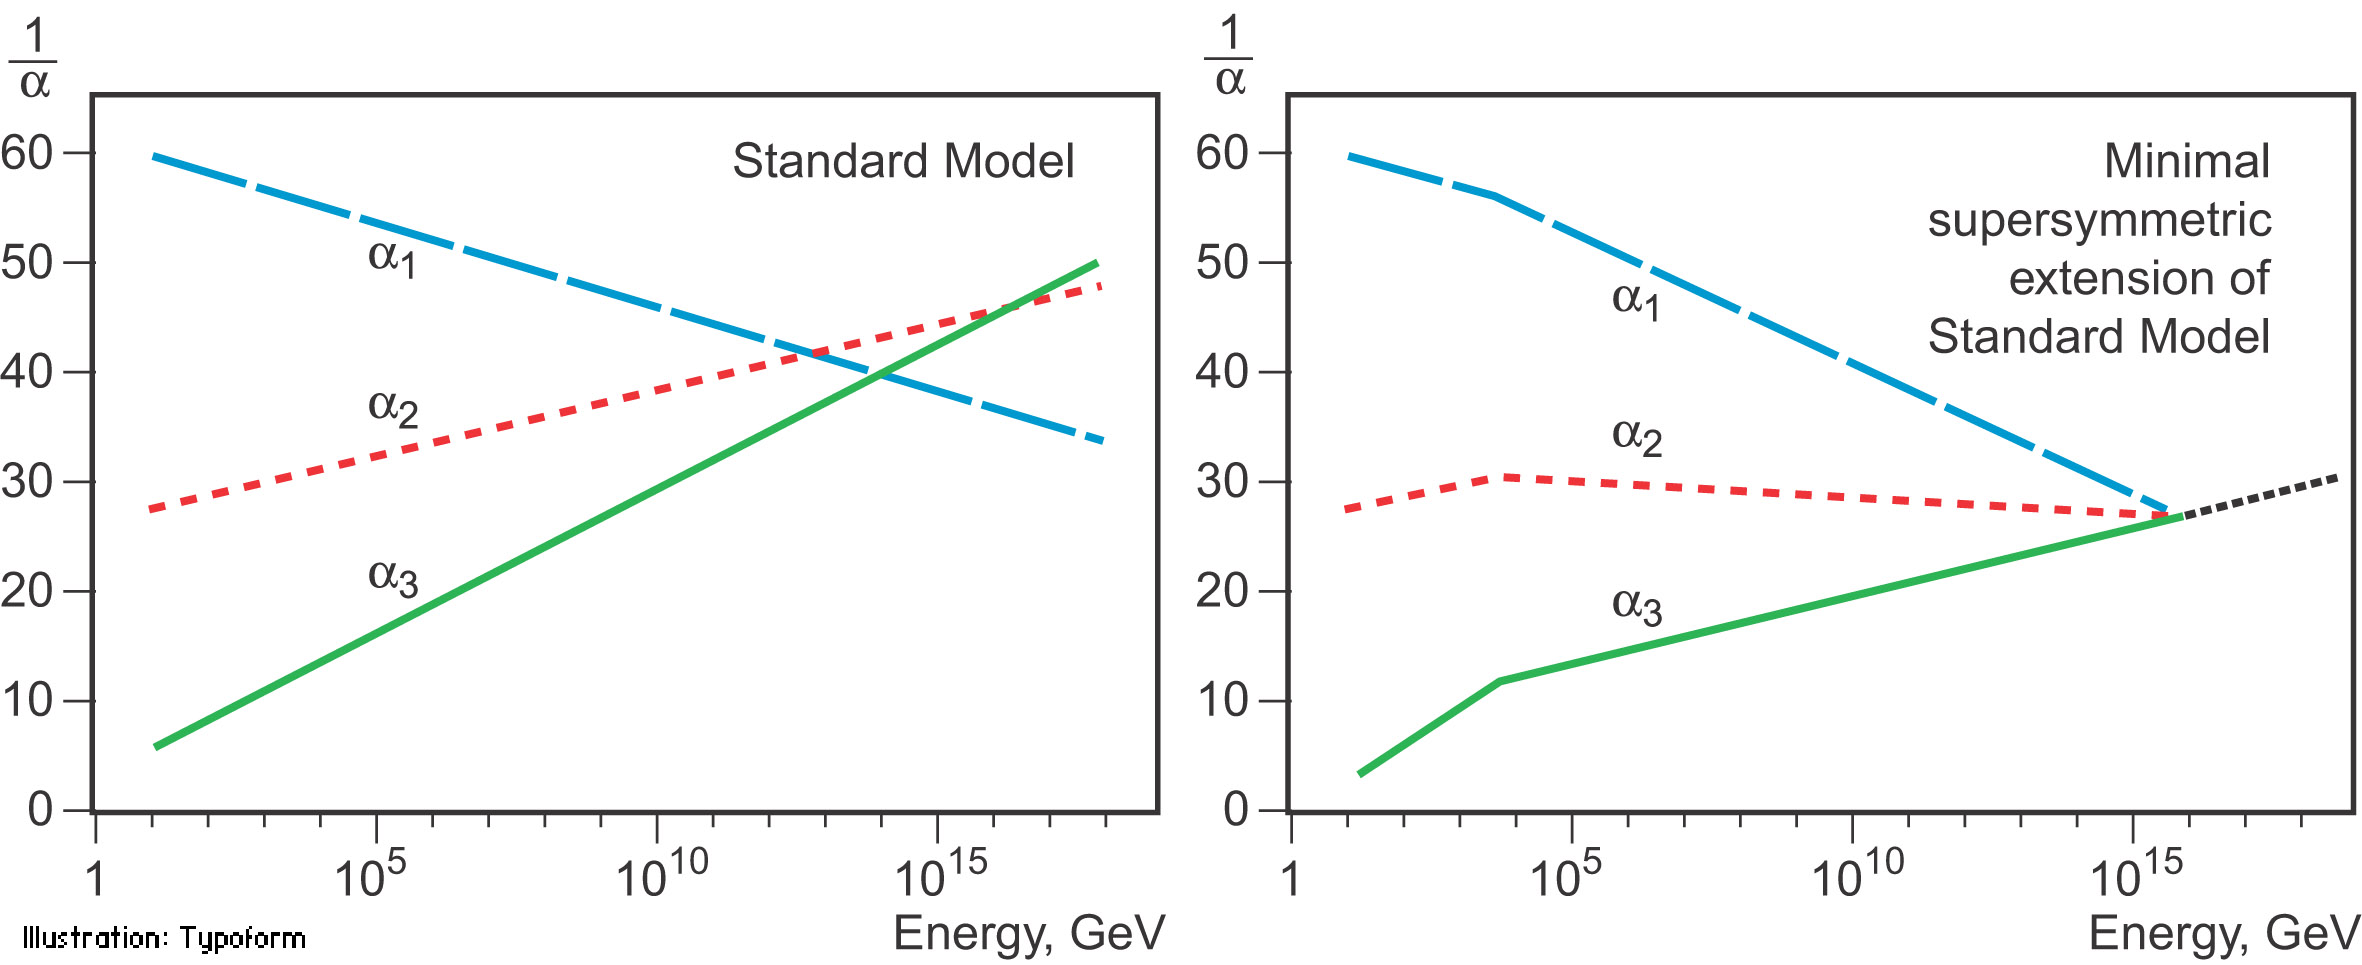
\includegraphics[width=\textwidth]{Figures/SM_MSSM.jpg}
	\caption{Here, $\alpha_1$, $\alpha_2$ and $\alpha_3$ represent the coupling constants of $U_Y(1)$, $SU_L(2)$ and $SU_{color}(3)$, respectively. What is shown is the variation of the inverse of the coupling with the energy: on the left for the SM and on the right for the MSSM. Plots from Ref. \cite{running_coupling}.}
	\label{fig:SM_MSSM}
\end{figure}

An early proposal of a theory that could unify gravity with electromagnetism was given by Theodore Kaluza in 1921. In particular, he showed that these two forces could stem from a single tensor with the introduction of an extra space dimension. In 1926, Oscar Klein offered an explanation for this extra dimension; he proposed that it had a circular topology such that at each point of the four dimensional space-time we would have a circle with a small radius. This theory has more degrees of freedom (because it is formulated in a higher dimensional space-time) and therefore it predicts new particles that are usually known as Kaluza-Klein gravitons (and their excited states). Nonetheless, the Kaluza-Klein model does not provide a satisfactory explanation for the hierarchy problem. Therefore, in 1999, Lisa Randall and Raman Sundrum introduced a new model that does. This model introduces only two new particles: a spin 2 graviton (and its Kaluza-Klein excitations) and a radion, that is a spin 0 neutral particle.

Models with two Higgs doublets (2HDM) are one of the simplest possible extensions of the Higgs sector of the SM. They are appealing because while the fermionic sector is rather complex, having three families, the scalar sector is quite simple, having a single particle, which seems unnatural. This type of structure is realized in various new physics models including SUSY models. In addition, they provide an additional source for CP violation which could help explain the matter-anti-matter asymmetry in the Universe. 

The most general renormalizable 2HDM scalar potential is written as \cite{2HDMpedro}
\begin{align}
	V&=m_{11}^2 |\Phi_1|^2+m_{22}^2 |\Phi_2|^2-(m_{12}^2 \Phi_1^{\dagger}\Phi_2+h.c.)\nonumber \\
	&+\frac{1}{2}\lambda_1|\Phi_1|^4+\frac{1}{2}\lambda_2|\Phi_2|^4+\lambda_3|\Phi_1|^2|\Phi_2|^2+\lambda_4|\Phi_1^{\dagger}\Phi_2|^2 \nonumber \\
	&+\left[\frac{1}{2}\lambda_5\left(\Phi_1^{\dagger}\Phi_2\right)^2+\lambda_6 |\Phi_1|^2\left(\Phi_1^{\dagger}\Phi_2\right)^2+\lambda_7 |\Phi_2|^2\left(\Phi_1^{\dagger}\Phi_2\right)^2+h.c.\right],	
	\label{eq:2HDMpot}
\end{align}  
where $\Phi_1$ and $\Phi_2$ are hypercharge doublets and the coefficients $m_{12}^2$ and $\lambda_{5,6,7}$ can be complex. However, when including the Yukawa interactions, the most general lagrangian leads to tree-level flavor changing neutral currents (FCNC) in the Yukawa sector. These FCNC are very tightly constrained by experimental data and should be avoided. They can be eliminated by imposing a $\mathbb{Z}_2$ symmetry. Although, usually, this symmetry is allowed to be softly broken in order to allow the theory to have a decoupling limit \cite{2HDMdec} where the mass of all the scalars other than the SM-like one can be made very large. In addition to the softly-broken $\mathbb{Z}_2$ symmetry, which leads to $\lambda_{6,7}=0$, we also impose CP conservation which makes all possible complex phases vanish. In this case, we obtain five Higgs bosons that are CP eigenstates. Three of them are neutral, $h$, $H$ and $A$, and the other two are charged, $H^{\pm}$. $h$ and $H$ are CP-even states while $A$ is CP-odd. $h$ is usually taken to be the SM Higgs boson and its mass is set to $125$ GeV.

There are several types of 2HDM classified according to their fermion-scalar interactions. We highlight the type II (the one used in this work), where all right-handed up-type quarks couple to $\Phi_2$ and right-handed down-type quarks and charged leptons couple to $\Phi_1$. This type of couplings is analogous to what happens in SUSY models. 

Instead of the parameters in Eq. \ref{eq:2HDMpot}, we can describe the model in terms of the four physical masses, $m_h$, $m_H$, $m_A$ and $m_{H^{\pm}}$, the angles $\alpha$ and $\beta$, the VEV $v=246$ GeV and a further parameter, chosen to be $m_{12}^2$ \cite{2HDMpedro}. The angle $\beta$ is defined as $\tan(\beta)=v_2/v_1$, where $v_{1,2}$ are the VEVs of the two Higgs doublets. The angle $\alpha$ diagonalizes the square mass matrix of the CP-even states. The quartic couplings of the potential can then be writen in terms of these parameters, as can be found in Eq. 11 of Ref. \cite{2HDMpedro}.

Simplified dark matter (DM) models are based on the exchange of a single particle between DM and SM particles and try to explain the nature of DM and how it interacts with the SM. The particle exchanged is called a mediator and, depending on the specific model, it can be neutral or electrically charged and have spin 0, 1 or 2. The simplest possible scenario is a neutral scalar mediator.

The CP-conserving 2HDM and dark matter model with a spin 0 mediator are explored in this work as sources of alternative di-Higgs production processes. For these models, the main modification with respect to the SM occurs because new heavy particles, namely, $H$ and the DM mediator can couple to the Higgs bosons through the s-channel diagram. This corresponds to replacing the off-shell Higgs boson by one of these particles in the Feynman diagram on the right in figure \ref{fig:higgs_pair}.

The spin-2 graviton predicted by Kaluza-Klein and Randal-Sundrum models can couple directly to gluons and then decay producing a Higgs pair, as it illustrated in figure \ref{fig:BSM_diag}(a). SUSY particles can contribute to the quantum loops in the Higgs production Feynamn diagrams. An example is shown in figure \ref{fig:BSM_diag}(b), where the top quark is replaced by its supersymmetric partner is the s-channel diagram. These are two other examples of how BSM models can change the Higgs pair production process with respect to the SM. 

The crucial point is that some BSM contributions can lead to an enhancement of the cross section for Higgs pair production with respect to what is predicted by the SM. Experimentally, this means that we would not need as much sensitivity and therefore the process could be measured with less data and therefore sooner. This is the reason why a lot of the searches performed at the LHC focus on this type of scenario. In addtion, if a new heavy particle couples to the Higgs boson via an s-channel diagram, it could lead to the existence of a peak in the Higgs pair invariant mass spectrum (assuming that we have enough experimental resolution and that there are not other processes coming into play). 

Moreover, BSM models introduce new free parameters (in addition to the SM ones) that can be constrained using the experimental results obtained at the LHC (and other experiments). This reduces the available parameter space of the models and may even reject some of them.

\begin{figure}
	\centering
	\begin{minipage}{.5\textwidth}
		\centering
		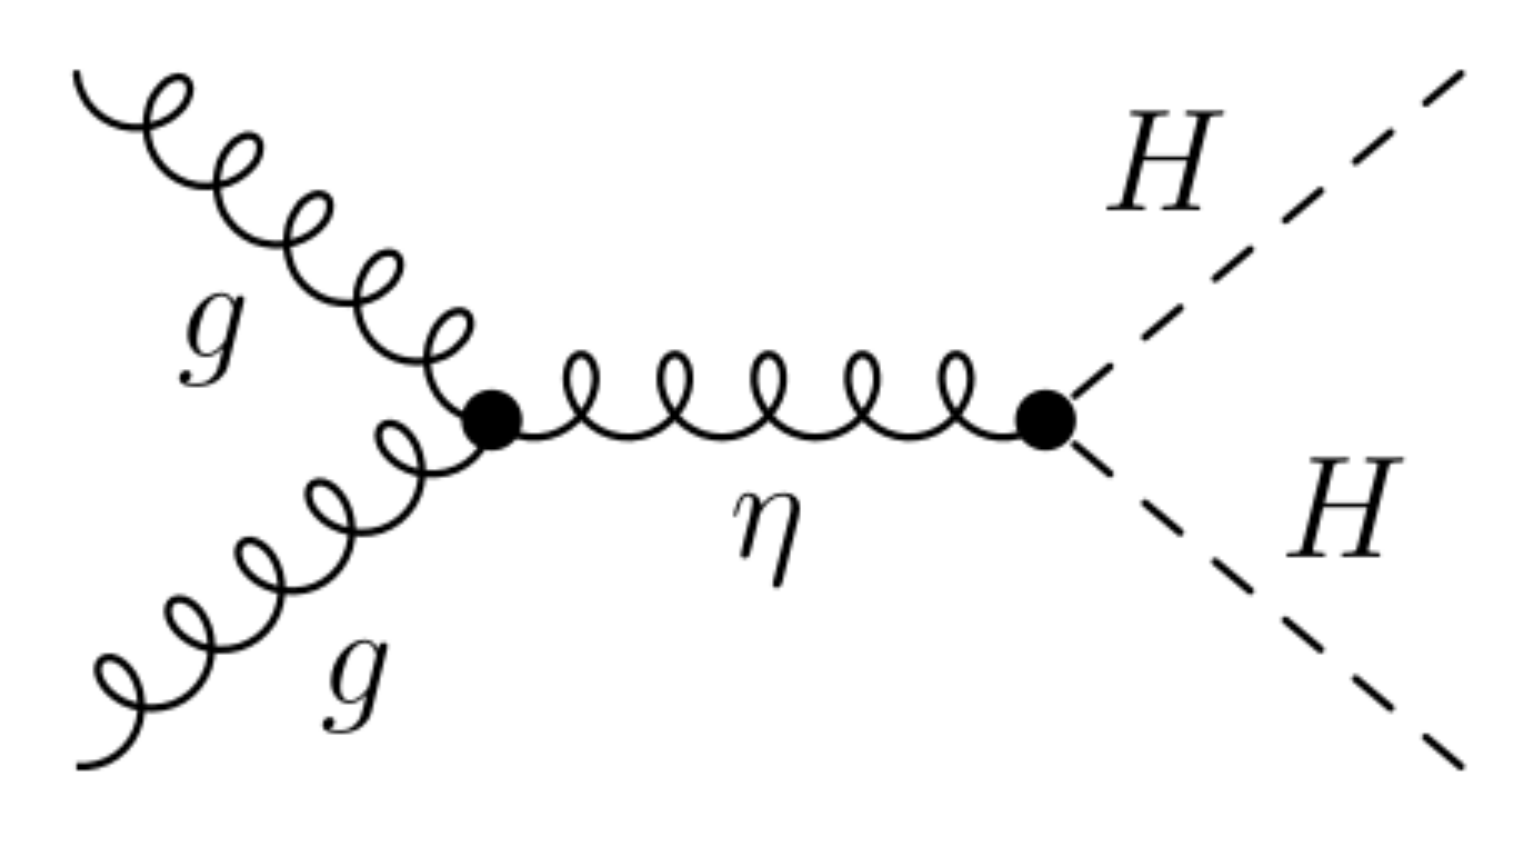
\includegraphics[trim={0cm 0cm 0cm 0cm},clip,width=.7\linewidth]{./Figures/graviton.png}
	\end{minipage}%
	\begin{minipage}{.5\textwidth}
		\centering
		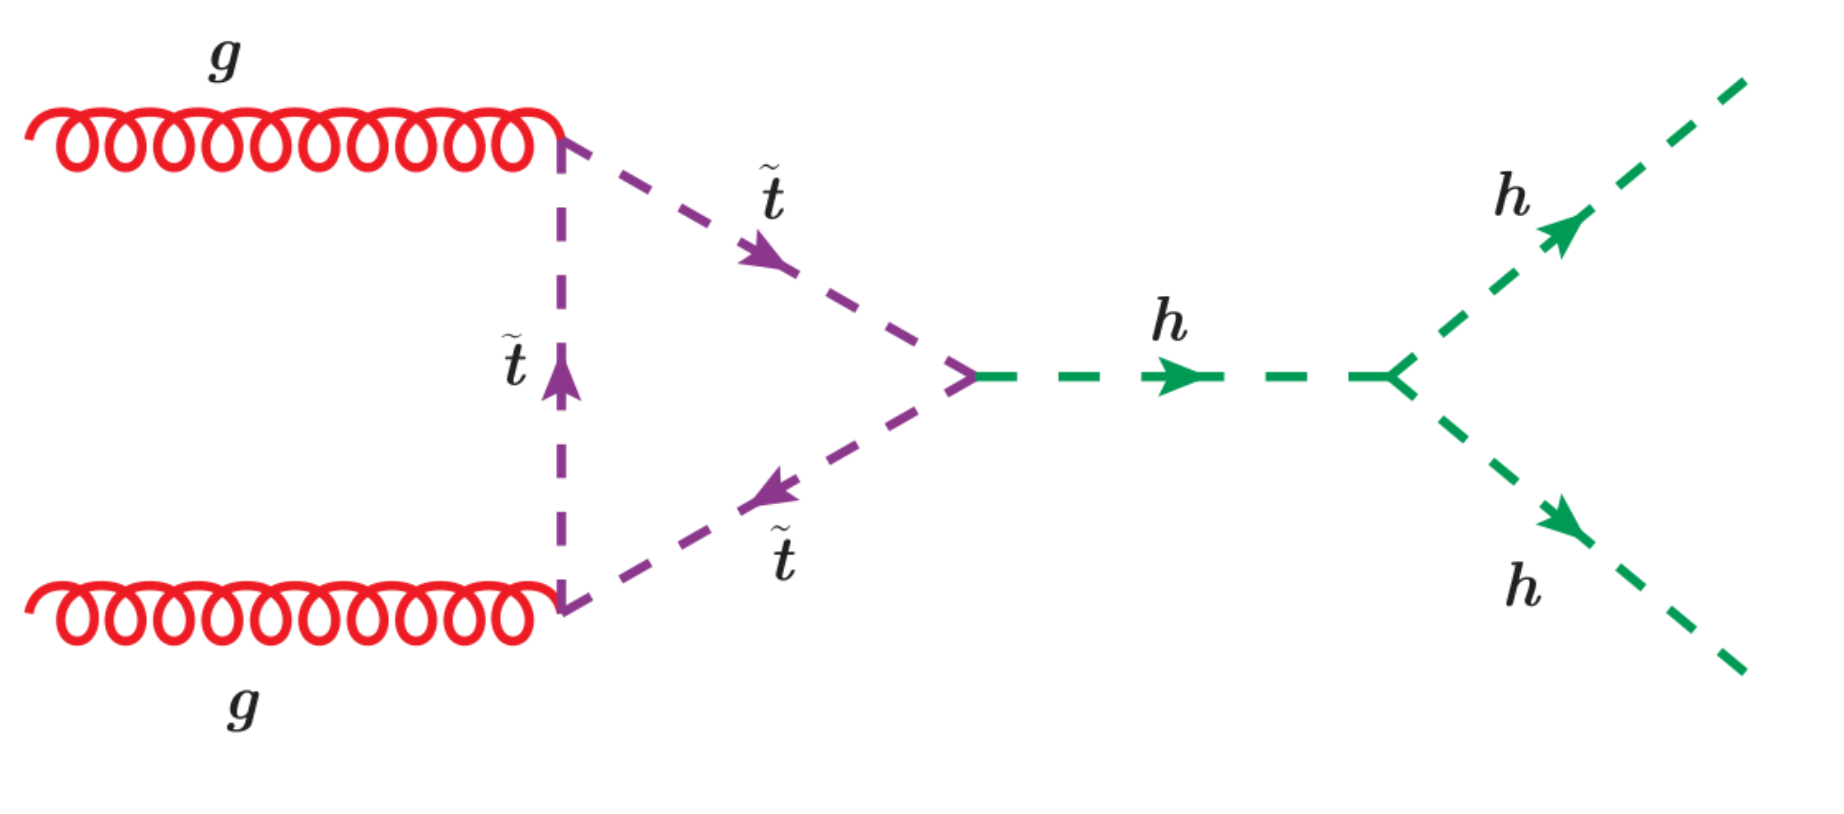
\includegraphics[trim={0cm .5cm 0cm 0cm},clip,width=\linewidth]{./Figures/susy.png}
	\end{minipage}
	\begin{minipage}[t]{0.5\textwidth}
		\caption*{(a)}
		%\label{fig1}
	\end{minipage}%%%
	\hfill
	\begin{minipage}[t]{0.5\textwidth}
		\caption*{(b)}
		%\label{fig2}
	\end{minipage}
	\caption{BSM contributions to Higgs pair production from the spin-2 Kaluza-Klein graviton (a) and from the SUSY partner of the top quark (b). Figures from Refs. \cite{hhBSMgrav,hhBSMsusy}, respectively.}
	\label{fig:BSM_diag}
\end{figure}

%BSM models: \cite{BSM_motivation}\\
%- GUT \\
%- SUSY \\
%- Large extra dimensions (Kaluza-Klein graviton) \\
%- Composite Higgs \\
%- Multi-Higgs 

%%%%%%%%%%%%%%%%%%%%%%%%%%%%%%%%%%%%%%%%%%%%%%%%%%%%%%%%%%%%%%%%%%%%%%%%
